\section{Model Averaging and Selection}\label{sec:Models}

\added{In many voxels, it is unclear how many fiber directions are supported by the data, i.e., which rank $r$ should be selected in Eq.~(\ref{eq:low-rank}). Selecting the most likely number incurs the risk of underestimating $r$, which could lead to premature termination of a secondary tract. On the other hand, overestimating $r$ confounds the tracking with spurious directions and increases the variance of the true fiber estimates. The idea behind model averaging is that smoothly blending between models, as it is illustrated in Figure~\ref{fig:base_overview}, should reduce the risk of missing an important fiber, while still relying on the more robust single-fiber estimates in regions that clearly do not support a larger number of directions. We implement this idea based on Bayesian model comparison (Section~\ref{sec:model-comparison}), and derive specific model averaging and model selection approaches in Section~\ref{sec:computing-tracking-directions}.}

\subsection{Model Comparison in a Bayesian Framework}
\label{sec:model-comparison}
In Bayesian model comparison, we are interested in the
posterior probability $p \left( \mathcal{H}_r \mid \mathcal{T} \right)$, where
$\mathcal{H}_r$ denotes the hypothesis that extracting $r$ fibers is optimal for a given fODF $\mathcal{T}$. Using Bayes' theorem of
conditional probability, \added{up to a common factor that we account for by a final re-normalization,} the posterior probability can be rewritten as
\begin{align}
	p \left( \mathcal{H}_r \mid \mathcal{T} \right) \propto p \left(
		\mathcal{T} \mid \mathcal{H}_r 
	\right) p \left(  \mathcal{H}_r \right), 
	\label{eq:Bayes}
\end{align}
where $p \left(  \mathcal{H}_r \right)$ is our prior belief that rank $r$ is
suitable, without considering the fODF. Since literature values for the prevalence of different $r$ over the white matter vary  \cite{BEHRENS2007144,Jeurissen:2012, Schultz:MICCAI12}, we use a
non-informative prior that assigns equal prior probability to the values of $r
\in \left\{ 1,2,3 \right\}$. The case $r=0$ can be excluded since we limit
tracking to a white matter mask.

The factor $p \left( \mathcal{T} \mid \mathcal{H}_r \right)$ is the
probability of the fODF $\mathcal{T}$ given a rank $r$. In the context of
Bayesian model comparison, it is referred to as model evidence. It is derived from $p
\left( \mathcal{T} \mid \mathcal{H}_r , \Theta_r \right)$, the posterior
probability of $T$ given an $r$-fiber model with a specific parameter vector
$\Theta_r$. In our case, $\Theta_r$ contains the variables from Eq.
(\ref{eq:low-rank}), i.e., $\Theta_r \coloneqq \left( \lambda_1 , \mathbf{v}_1 , \dots
, \lambda_r , \mathbf{v}_r \right)$. 

The overall model evidence is obtained by marginalization over parameter values,
\begin{align}
	p \left( \mathcal{T} \mid \mathcal{H}_r \right) = \int p \left(
		\mathcal{T} \mid \mathcal{H}_r , \Theta_r 
	\right) p \left( \Theta_r \mid \mathcal{H}_r  \right) d \Theta_r. 
	\label{eq:model-evidence}
\end{align}

Since a direct calculation of Eq. (\ref{eq:model-evidence}) would require solving a
high dimensional integral, we use an approximation via the Bayesian Information
Criterion
\[ \text{BIC} = k \ln \left( n \right) - 2 \ln \left( p \left( \mathcal{T} \mid
\mathcal{H}_r, \hat{\Theta}_r \right) \right), \]
where $p \left(  \mathcal{T} \mid \mathcal{H}_r , \hat{\Theta}_r \right)$
corresponds to the likelihood of the rank-$r$ with parameters $\hat{\Theta}_r$
that best fit the fODF $\mathcal{T}$, $k$ is the number of parameters in
$\Theta_r$, and $n$ denotes the number of data points to which the model was
fitted \cite{Schwarz1978}. We note that $k=3r$ increases with $r$, which penalizes the choice of multiple fibers, unless it leads to a sufficient increase of $p \left(  \mathcal{T} \mid \mathcal{H}_r , \hat{\Theta}_r \right)$. Under certain conditions, the BIC is related to the
model evidence by \cite{Konishi2008}
\begin{align}
	p \left( \mathcal{T} \mid \mathcal{H}_r \right) \approx \exp \left(  -
		\frac{\text{BIC}}{2}
\right).
	\label{eq:BIC-model}
\end{align}

% \subsection{From Model Likelihood to Model Uncertainty}
This allows us to compute the model evidence in a simple and efficient way.
However, we still need to provide an equation for $p
\left( \mathcal{T} \mid \mathcal{H}_r , \hat{\Theta}_r \right)$. Therefore, we
use the relative magnitude of the corresponding low-rank approximation residual 
\begin{align}
	\| \tilde{\mathcal{R}}^{\left( r \right)} \| = \frac{ \| \mathcal{T} -
	\mathcal{T}^{\left( r \right)} \| }{ \| \mathcal{T} \|} \in \left[ 0,1
	\right],
	\label{eq:residual}
\end{align}
since a smaller residual from a rank-$r$ approximation should indicate a higher probability of $\mathcal{T}$ being a perturbation of a rank-$r$ tensor. Since many factors contribute to the magnitude of this residual, including measurement noise, fiber spread, and inaccuracies in the convolution kernel, we pragmatically model
$p
\left( \mathcal{T} \mid \mathcal{H}_r , \hat{\Theta}_r \right)$ with the computationally efficient Kumaraswamy Probability Density Function (PDF) \cite{Kumaraswamy1980}

\begin{align}
	f \left( x, a, b \right) \coloneqq ab x^{a-1} \left( 1- x^a
	\right)^{b-1} \text{ for } x \in \left( 0,1 \right) \text{ and } a,b >
	0
	\label{eq:Kumaraswamy}
\end{align}
which is defined on the correct interval $(0,1)$, and can be tuned to achieve
the correct qualitative behavior \added{of monotonically decreasing with increasing $\|
  \tilde{\mathcal{R}}^{\left( r \right)} \|$ by setting $a=1, b>2$.}

\begin{figure}
	\centering
	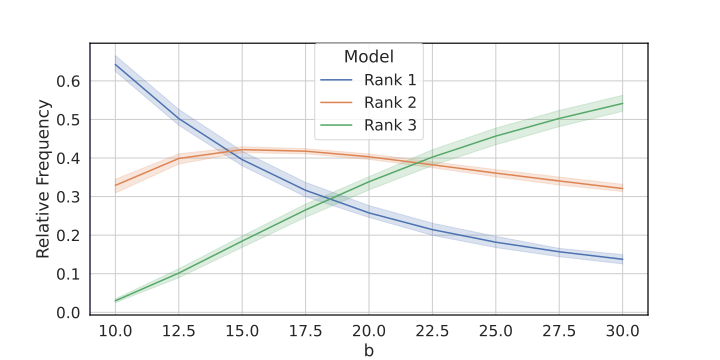
\includegraphics[width=\linewidth]{b_check}
	\caption{\added{Relative frequency of selecting ranks $\left\{ 1,
              2,3 \right\}$ within a white matter mask based on the Kumaraswamy PDF with $a=1$ and different values of $b$. The lines indicate the mean over all subjects from Section~\ref{sec:data}, the tubes the minimum and maximum.}}
	\label{fig:b}
\end{figure}

\added{With increasing $b$, the probability decreases at steeper slopes. As
illustrated in Figure~\ref{fig:b}, this favors modelling larger numbers of
fibers, since that permits a reduction of fitting residuals. Thus, the choice of
$b$ can be seen as determining how strong the support for a secondary or
tertiary compartment needs to be so that it will be used for tracking. Having to
make this decision is a source of uncertainty in all methods for crossing fiber
tractography, and has contributed to the variability in literature values on the
prevalence of two- and three-fiber voxels \cite{BEHRENS2007144,Jeurissen:2012,
Schultz:MICCAI12}. In our experiments, we set $b=20$, which leads to values
within the range of literature values. We expect that the normalization that
results from deconvolving with subject-specific response functions
\cite{Jeurissen:2014} and the normalization in Eq.~(\ref{eq:residual}) will
allow for similar choices of $b$ across datasets. This is supported by the
relatively narrow confidence intervals across subjects in Figure~\ref{fig:b}.}

\subsection{Computing Tracking Directions from Alternative Models}
\label{sec:computing-tracking-directions}

As in our previous work \cite{Gruen:2021}, we fuse the information from tensor
approximations with different ranks $r \in \left\{ 1,2 , 3 \right\}$ by taking a weighted sum of the
corresponding parameters $\mathbf{v}_i^{\left( r \right)}$ and
$\lambda_i^{\left( r \right)}$ with weights given by the above-defined posterior probabilities. We refer to this strategy as \emph{model averaging.}

Before computing the weighted sum, we have to establish a correspondence between the directions of the
different $r$-fiber models. In other words, we have to re-order the directions from each rank $r$ such that the first directions of the two- and three-fiber models are matched with the direction from the single fiber model, and that the second directions of the two- and three-fiber models match. This leads to $2! \times 3! =12$ possible assignments, from which we
select the one that minimizes the overall sum of angles between the resulting
weighted means $\mathbf{v}_i$ and their corresponding $\mathbf{v}_i^{\left( r
\right)}$.

\added{A potential objection against the idea of model averaging is that, in case multiple probable models should yield very dissimilar directions, averaging them might produce spurious directions that did not occur in any of the original models. Therefore, we computed the smallest distances between the main direction of the average model and the closest direction of the corresponding low-rank models
	within the white matter mask of a randomly chosen subject from the
	experiment in Section \ref{sec:data}. In $95\%$ of all white matter
	voxels, that angle was below $1.8^{\circ}$. Since that is well below the
        angular resolution of CSD \cite{Ankele:CARS2017}, we conclude that,  in practice, corresponding directions are similar enough that it is reasonable to average them.} 

Previous tractography algorithms that were based on low-rank tensor approximation \cite{Ankele:CARS2017} used a different strategy, that we refer to as \emph{model selection:} They determined an optimal rank $r \in \left\{ 1, \added{2}, 3 \right\}$ in each integration step and used the resulting set of
directions $\mathbf{v}_i$ for tracking. In cases where several ranks have non-negligible probabilities, this introduces an uncertainty that model averaging aims to reduce. We include this approach
as a baseline in our experiments. To enable a direct comparison, we select the model with the highest probability $p \left(
 \mathcal{H}_r \mid \mathcal{T} \right)$ according to the same Bayesian framework.
 

%%% Local Variables:
%%% mode: latex
%%% TeX-master: "../main"
%%% End:
